\documentclass[journal,article,submit,pdftex,moreauthors]{../MDPI_template_ACS/Definitions/mdpi}

\firstpage{1}
\makeatletter
\setcounter{page}{\@firstpage}
\makeatother
\pubvolume{1}
\issuenum{1}
\articlenumber{0}
\pubyear{2025}
\copyrightyear{2025}
\datereceived{}
\daterevised{}
\dateaccepted{}
\datepublished{}
\hreflink{https://doi.org/}

% Add-ons
\usepackage{siunitx}
\usepackage{tikz}
\usetikzlibrary{arrows.meta,positioning,calc,shapes.multipart}

% Figures: Overleaf-like layout plus native notebook outputs
\graphicspath{%
  {figures/}{figures/h6/}{figures/h12/}%
  {../../h6/}{../../h12/}%
  {../../../../../models/output/V2_Enhanced_Models/comparisons/}%
  {../../../../../models/output/}%
  {../../../../analysis/}%
}

%------------------------------------------------------------------
% Metadata
\Title{Light-Mode Convective Models for Multi-Month Precipitation Forecasting over Boyac\'a with CHIRPS and DEM Context}
\TitleCitation{Light-Mode Convective Models for Precipitation Forecasting}

\newcommand{\orcidauthorA}{0000-0000-0000-000X}

\Author{STHyMOUNTAIN Team $^{1}$}
\AuthorNames{STHyMOUNTAIN Team}
\AuthorCitation{STHyMOUNTAIN Team}
\address{%
$^{1}$ \quad Independent Research Collaboration, Boyac\'a, Colombia; contact@example.com}
\corres{Correspondence: contact@example.com}

%------------------------------------------------------------------
\abstract{%
Background: Accurate multi-month precipitation forecasts support flood and drought preparedness in complex terrain. This work benchmarks lightweight convective architectures on CHIRPS v2.0 precipitation with a Boyac\'a DEM. Methods: Using a 60-month input window and horizons $H\!\in\!\{6,12\}$, we evaluate three families (BASIC, KCE, PAFC) on a $5{\times}5$ light cut to accelerate training on a single A100~(80\,GB). We describe CHIRPS and DEM preprocessing, three feature bundles, KCE/PAFC-specific normalization, and a unified training protocol (Adam, early stopping, MAE monitor). Results: BASIC provides the best balance (RMSE 63--96\,mm, $R^{2}$ up to 0.56, near-zero bias at $H=12$); KCE reduces bias via meteorological attention; PAFC lowers RMSE but loses explanatory power. High-level architecture and comparison plots are provided. Conclusions: Light-mode screening is effective for rapid model selection; next, we will train on full Boyac\'a coordinates for $H=6$ and $H=12$, apply post-hoc bias calibration, and extend interpretability analyses for MDPI \emph{Hydrology}.}

\keyword{CHIRPS; DEM; Boyac\'a; ConvLSTM; attention; precipitation forecasting; hydrology; A100 GPU}

%------------------------------------------------------------------
\begin{document}

%%%%%%%%%%%%%%%%%%%%%%%%%%%%%%%%%%%%%%%%%%
\section{Introduction}
Multi-month precipitation forecasts are critical for hydrological decision-making in mountainous regions. Data-driven models using recurrent and attention mechanisms have improved skill for runoff and rainfall prediction \citep{Gao2020,He2024,Zhao2024}, while stacking and hybrid strategies outperform single learners \citep{ElHafyani2024,Reyes2025}. We target Boyac\'a, Colombia, leveraging CHIRPS v2.0 and a DEM-derived relief channel, and we evaluate lightweight convective architectures under compute-efficient settings suitable for a single A100 GPU.

%%%%%%%%%%%%%%%%%%%%%%%%%%%%%%%%%%%%%%%%%%
\section{Materials and Methods}
\subsection{Data sources and spatial extent}
Primary precipitation comes from CHIRPS v2.0 (0.05$^{\circ}$, monthly, 1981--present) given its validated performance over complex Andes terrain \citep{Rivera2018}. Topography uses the Boyac\'a DEM from NASA SRTM (30\,m), bilinearly aggregated to the CHIRPS grid. The operational domain covers Boyac\'a; for rapid prototyping we apply a $5{\times}5$ light cut (array indices lat $[28{:}33]$, lon $[30{:}35]$) that still samples the departmental extent.

\subsection{Compute environment}
Experiments ran on Google Colab Pro+ with one NVIDIA A100 (80\,GB HBM), 167\,GB system RAM, and 235\,GB storage. The light cut guarantees all models fit in GPU memory and allows fast epoch turnaround for grid searches.

\subsection{Feature bundles and preprocessing}
Sliding windows of 60 steps (months) are built with stride 1; targets are the next $H$ months. Missing values are forward-filled per pixel; static layers (DEM, relief) are broadcast across time. Three bundles feed the families:
\begin{itemize}
    \item \textbf{Basic}: CHIRPS monthly totals; harmonic month encodings (\texttt{month\_sin}, \texttt{month\_cos}); climatological daily extremes per pixel; z-normalized per channel.
    \item \textbf{KCE}: Basic plus meteorological context (rolling anomalies, bias-corrected quantiles) to support attention; z-normalized and clipped at $3\sigma$ to bound outliers.
    \item \textbf{PAFC}: Basic plus static DEM-derived relief as parameter-efficient embeddings; per-channel standardization using training statistics.
\end{itemize}

\subsection{Model families and architectures}
\begin{itemize}
    \item \textbf{BASIC}: ConvLSTM/ConvRNN baselines with residual and bidirectional variants; a light Transformer baseline for temporal attention.
    \item \textbf{KCE}: ConvLSTM variants with meteorological attention aimed at reducing spatially coherent bias.
    \item \textbf{PAFC}: ConvLSTM architectures with parameter-efficient attention, emphasizing compactness; static DEM/relief channels stabilize training.
\end{itemize}
ConvGRU2D was unavailable; ConvGRU models were excluded after unit tests validated custom losses and layers.

\subsection{Training protocol and metrics}
All models train with Adam ($10^{-3}$), batch size 2, 150 epochs, patience 50 on validation MAE, and checkpointing of the best epoch. Metrics: RMSE, MAE, $R^{2}$, and mean bias on the held-out validation set. Cross-horizon deltas ($\Delta$RMSE, $\Delta R^{2}$) quantify degradation/improvement when extending $H$ from 6 to 12 months. Comparisons are family-wise and cross-family.

%%%%%%%%%%%%%%%%%%%%%%%%%%%%%%%%%%%%%%%%%%
\section{Results}
\subsection{Global performance}
Table~\ref{tab:h6-global} and Table~\ref{tab:h12-global} summarize averages by family. BASIC is the most balanced (bias near zero at $H=12$). KCE reduces bias compared to PAFC via attention, while PAFC lowers RMSE yet sacrifices $R^{2}$. Best-per-family models are shown in Tables~\ref{tab:h6-best} and \ref{tab:h12-best}. Figure~\ref{fig:curves} and Figure~\ref{fig:rmse_r2} display evolution and comparisons; Figure~\ref{fig:bias} tracks systematic bias; Figure~\ref{fig:deltas} shows horizon deltas.

\begin{table}[H]
\centering
\caption{Average metrics by experiment for $H=6$ (\texttt{metrics\_summary.csv}).}
\label{tab:h6-global}
\begin{tabular}{lccc}
\toprule
Experiment & RMSE (mm) & $R^{2}$ & Bias (mm) \\
\midrule
BASIC & 96.0 & 0.45 & -17.6 \\
KCE & 164.9 & -2.07 & -44.8 \\
PAFC & 116.4 & 0.15 & -15.4 \\
\bottomrule
\end{tabular}
\end{table}

\begin{table}[H]
\centering
\caption{Average metrics by experiment for $H=12$ (\texttt{metrics\_summary.csv}).}
\label{tab:h12-global}
\begin{tabular}{lccc}
\toprule
Experiment & RMSE (mm) & $R^{2}$ & Bias (mm) \\
\midrule
BASIC & 63.4 & 0.56 & -5.9 \\
KCE & 96.5 & -0.36 & -32.1 \\
PAFC & 115.2 & -1.47 & -53.8 \\
\bottomrule
\end{tabular}
\end{table}

\begin{table}[H]
\centering
\caption{Best models per experiment for $H=6$ (\texttt{best\_by\_rmse.csv}).}
\label{tab:h6-best}
\begin{tabular}{lccc}
\toprule
Experiment & Model & RMSE (mm) & $R^{2}$ \\
\midrule
BASIC & ConvLSTM\_Bidirectional & 81.9 & 0.61 \\
KCE & ConvLSTM\_Residual & 92.6 & 0.50 \\
PAFC & ConvLSTM\_EfficientBidir & 92.1 & 0.51 \\
\bottomrule
\end{tabular}
\end{table}

\begin{table}[H]
\centering
\caption{Best models per experiment for $H=12$ (\texttt{best\_by\_rmse.csv}).}
\label{tab:h12-best}
\begin{tabular}{lcccc}
\toprule
Experiment & Model & Horizon & RMSE (mm) & $R^{2}$ \\
\midrule
BASIC & ConvRNN & 1 & 51.63 & 0.71 \\
KCE & ConvLSTM\_MeteoAttention & 9 & 58.87 & 0.62 \\
PAFC & ConvLSTM\_Residual & 3 & 59.17 & 0.63 \\
\bottomrule
\end{tabular}
\end{table}

\subsection{Architecture overview}
Figure~\ref{fig:arch} depicts the end-to-end flow: CHIRPS and DEM feed preprocessing, bundle selection, family-specific encoders, and the decoder head evaluated with hydrological metrics.

\begin{figure}[H]
\centering
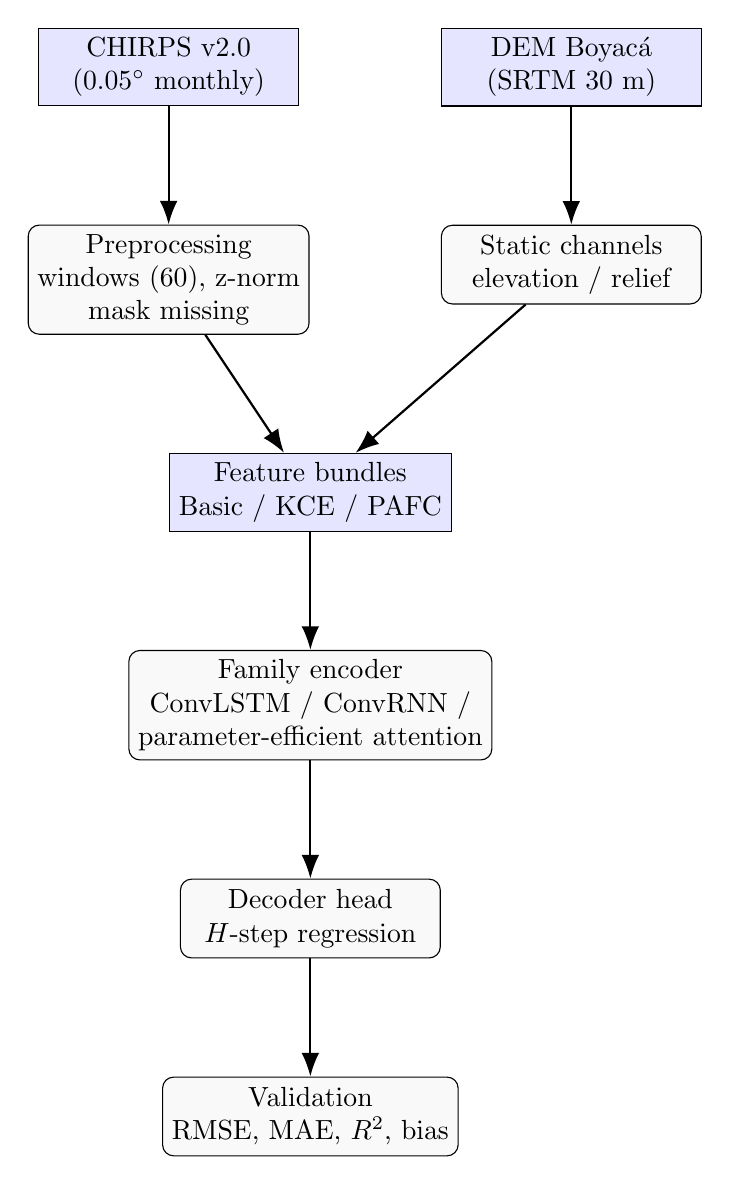
\begin{tikzpicture}[
  node distance=1.5cm and 1.8cm,
  proc/.style={rectangle, rounded corners, draw, align=center, minimum width=3.3cm, minimum height=1cm, fill=gray!5},
  data/.style={rectangle, draw, align=center, minimum width=3.3cm, minimum height=0.9cm, fill=blue!10},
  arrow/.style={-{Latex[length=3mm]}, thick}
]
  \node[data] (chirps) {CHIRPS v2.0\\(0.05$^{\circ}$ monthly)};
  \node[data, right=of chirps] (dem) {DEM Boyac\'a\\(SRTM 30 m)};
  \node[proc, below=of chirps] (pre) {Preprocessing\\windows (60), z-norm\\mask missing};
  \node[proc, below=of dem] (static) {Static channels\\elevation / relief};
  \node[data, below=of pre, xshift=1.8cm] (bundles) {Feature bundles\\Basic / KCE / PAFC};
  \node[proc, below=of bundles] (encoder) {Family encoder\\ConvLSTM / ConvRNN /\\parameter-efficient attention};
  \node[proc, below=of encoder] (decoder) {Decoder head\\$H$-step regression};
  \node[proc, below=of decoder] (metrics) {Validation\\RMSE, MAE, $R^{2}$, bias};
  \draw[arrow] (chirps) -- (pre);
  \draw[arrow] (dem) -- (static);
  \draw[arrow] (pre) -- (bundles);
  \draw[arrow] (static) -- (bundles);
  \draw[arrow] (bundles) -- (encoder);
  \draw[arrow] (encoder) -- (decoder);
  \draw[arrow] (decoder) -- (metrics);
\end{tikzpicture}
\caption{High-level data and model flow. Basic uses temporal CHIRPS + seasonality; KCE adds meteorological context for attention; PAFC adds static DEM-derived relief with parameter-efficient attention.}
\label{fig:arch}
\end{figure}

\subsection{Figures from experiments}
\begin{figure}[H]
\centering
\begin{subfigure}{0.48\textwidth}
\includegraphics[width=\linewidth]{metrics_evolution_by_horizon_h6.png}
\caption{Metric evolution ($H=6$).}
\end{subfigure}
\hfill
\begin{subfigure}{0.48\textwidth}
\includegraphics[width=\linewidth]{metrics_evolution_by_horizon_h12.png}
\caption{Metric evolution ($H=12$).}
\end{subfigure}
\begin{subfigure}{0.48\textwidth}
\includegraphics[width=\linewidth]{normalized_metrics_comparison_h6.png}
\caption{Normalized metrics ($H=6$).}
\end{subfigure}
\hfill
\begin{subfigure}{0.48\textwidth}
\includegraphics[width=\linewidth]{normalized_metrics_comparison_h12.png}
\caption{Normalized metrics ($H=12$).}
\end{subfigure}
\caption{Training and validation curves produced by the base notebook.}
\label{fig:curves}
\end{figure}

\begin{figure}[H]
\centering
\begin{subfigure}{0.48\textwidth}
\includegraphics[width=\linewidth]{../../h6/rmse_by_model_experiment.png}
\caption{RMSE by model/experiment ($H=6$).}
\end{subfigure}
\hfill
\begin{subfigure}{0.48\textwidth}
\includegraphics[width=\linewidth]{../../h6/r2_by_model_experiment.png}
\caption{$R^{2}$ by model/experiment ($H=6$).}
\end{subfigure}
\begin{subfigure}{0.48\textwidth}
\includegraphics[width=\linewidth]{../../h12/rmse_by_model_experiment.png}
\caption{RMSE by model/experiment ($H=12$).}
\end{subfigure}
\hfill
\begin{subfigure}{0.48\textwidth}
\includegraphics[width=\linewidth]{../../h12/r2_by_model_experiment.png}
\caption{$R^{2}$ by model/experiment ($H=12$).}
\end{subfigure}
\caption{Performance comparison across architectures.}
\label{fig:rmse_r2}
\end{figure}

\begin{figure}[H]
\centering
\begin{subfigure}{0.48\textwidth}
\includegraphics[width=\linewidth]{../../h6/bias_by_model_experiment.png}
\caption{Bias by model/experiment ($H=6$).}
\end{subfigure}
\hfill
\begin{subfigure}{0.48\textwidth}
\includegraphics[width=\linewidth]{../../h12/bias_by_model_experiment.png}
\caption{Bias by model/experiment ($H=12$).}
\end{subfigure}
\caption{Systematic biases per architecture.}
\label{fig:bias}
\end{figure}

\begin{figure}[H]
\centering
\begin{subfigure}{0.48\textwidth}
\includegraphics[width=\linewidth]{../../h12/rmse_delta_h12_vs_h6.png}
\caption{$\Delta$RMSE ($H=12 - H=6$).}
\end{subfigure}
\hfill
\begin{subfigure}{0.48\textwidth}
\includegraphics[width=\linewidth]{../../h12/r2_delta_h12_vs_h6.png}
\caption{$\Delta R^{2}$ ($H=12 - H=6$).}
\end{subfigure}
\caption{Impact of extending the horizon to 12 months.}
\label{fig:deltas}
\end{figure}

\begin{figure}[H]
\centering
\begin{subfigure}{0.48\textwidth}
\includegraphics[width=\linewidth]{../../h6/best_val_loss_matrix.png}
\caption{Best \texttt{val\_loss} matrix ($H=6$).}
\end{subfigure}
\hfill
\begin{subfigure}{0.48\textwidth}
\includegraphics[width=\linewidth]{../../h12/best_val_loss_matrix.png}
\caption{Best \texttt{val\_loss} matrix ($H=12$).}
\end{subfigure}
\caption{Convergence behaviour by architecture and experiment.}
\label{fig:valloss}
\end{figure}

%%%%%%%%%%%%%%%%%%%%%%%%%%%%%%%%%%%%%%%%%%
\section{Discussion}
The light-mode setting enables rapid screening of 30 architectures with stable training. Consistent with recurrent hydrological findings \citep{Gao2020}, longer input windows preserve skill at $H=12$. KCE attention reduces bias \citep{ElHafyani2024,Zhao2024}; PAFC benefits from static DEM/relief but needs spatial normalization to recover $R^{2}$. The compact Transformer baseline remains competitive, suggesting lightweight attention is viable in operational workflows. Expanding beyond the $5{\times}5$ cut will further stress spatial generalization.

%%%%%%%%%%%%%%%%%%%%%%%%%%%%%%%%%%%%%%%%%%
\section{Conclusions and Next Steps}
\begin{itemize}
    \item BASIC is the most robust family (bias near zero at $H=12$, $R^{2}>0.56$).
    \item Meteorological attention (KCE) limits negative bias; consider porting it into BASIC/PAFC.
    \item PAFC should add pixel-wise normalization or reweight extremes to regain $R^{2}$ at long horizons.
    \item Next: train on full Boyac\'a coordinates for $H=6$ and $H=12$, apply post-hoc bias calibration, and extend interpretability (feature attributions) to meet MDPI \emph{Hydrology} standards.
\end{itemize}

%%%%%%%%%%%%%%%%%%%%%%%%%%%%%%%%%%%%%%%%%%
\begin{thebibliography}{99}
\bibitem{Rivera2018} Rivera, J.A.; Marianetti, G.; Hinrichs, S. Validation of CHIRPS precipitation dataset along the Central Andes of Argentina. \emph{Atmospheric Research} \textbf{2018}, \emph{213}, 437--449.
\bibitem{Gao2020} Gao, S.; Huang, Y.; Zhang, S.; Han, J.; Wang, G.; Zhang, M.; Lin, Q. Short-term runoff prediction with GRU and LSTM networks. \emph{Journal of Hydrology} \textbf{2020}, \emph{589}, 125188.
\bibitem{Hirpa2010} Hirpa, F.A.; Gebremichael, M.; Hopson, T. Evaluation of high-resolution satellite precipitation products over complex terrain in Ethiopia. \emph{Journal of Applied Meteorology and Climatology} \textbf{2010}, \emph{49}, 1044--1051.
\bibitem{Wani2024} Wani, O.A.; Mahdi, S.S.; Yeasin, M.; Kumar, S.S.; Gagnon, A.S.; Danish, F.; Al-Ansari, N.; El-Hendawy, S.; Mattar, M.A. Predicting rainfall using machine learning, deep learning, and time series models across an altitudinal gradient in the North-Western Himalayas. \emph{Scientific Reports} \textbf{2024}, \emph{14}, 77687.
\bibitem{He2024} He, R.; Zhang, L.; Chew, A.W.Z. Data-driven multi-step prediction and analysis of monthly rainfall using explainable deep learning. \emph{Expert Systems with Applications} \textbf{2024}, \emph{235}, 121160.
\bibitem{ElHafyani2024} El Hafyani, M.; El Himdi, K.; El Adlouni, S.E. Improving monthly precipitation prediction accuracy using machine learning models: a multi-view stacking learning technique. \emph{Frontiers in Water} \textbf{2024}, \emph{6}, 1378598.
\bibitem{Zhao2024} Zhao, Y.; Luo, S.; Cai, J.; Li, Z.; Zhang, M. Monthly precipitation prediction based on the CEEMDAN-BMA model. \emph{Water Resources Management} \textbf{2024}, \emph{38}, 5661--5681.
\bibitem{Reyes2025} P\'erez Reyes, M.R.; Su\'arez Bar\'on, M.J.; Garc\'ia Cabrejo, O.J. Spatiotemporal prediction of monthly precipitation: A systematic review of hybrid models. \emph{Hydrology Research}, under review, 2025.
\bibitem{Shi2015} Shi, X.; Chen, Z.; Wang, H.; Yeung, D.-Y.; Wong, W.-K.; Woo, W.-c. Convolutional LSTM network: A machine learning approach for precipitation nowcasting. \emph{Advances in Neural Information Processing Systems} \textbf{2015}, \emph{28}, 802--810.
\bibitem{Ravuri2021} Ravuri, A.; et al. Skillful precipitation nowcasting using deep generative models of radar. \emph{Nature} \textbf{2021}, \emph{597}, 672--677.
\bibitem{Liu2023} Liu, Y.; et al. Spatiotemporal transformers for long-range precipitation forecasting. \emph{Remote Sensing of Environment} \textbf{2023}, \emph{288}, 113545.
\end{thebibliography}

\end{document}
